% Created 2018-09-30 Sun 16:29
% Intended LaTeX compiler: pdflatex
\documentclass[10pt,t]{beamer}
\usepackage[utf8]{inputenc}
\usepackage[T1]{fontenc}
\usepackage{graphicx}
\usepackage{grffile}
\usepackage{longtable}
\usepackage{wrapfig}
\usepackage{rotating}
\usepackage[normalem]{ulem}
\usepackage{amsmath}
\usepackage{textcomp}
\usepackage{amssymb}
\usepackage{capt-of}
\usepackage{hyperref}
\usetheme{default}
\author{L. Larrabee Strow}
\date{\today}
\title{\large A AIRS Plus CrIS/IASI Multi-Decadal Trends and Anomalies with Full Spatial Sampling and Rigorous Error Characterization}
\subtitle{\footnotesize{AIRS Science Team Meeting}}
\date{\vspace{0.1in}\footnotesize{April 25, 2018 \vfill}}
\author{L. Larrabee Strow\inst{1,2}, Sergio De-Souza Machado\inst{1,2}, Steven Leroy\inst{3}, Howard Motteler\inst{2}, Chris Hepplewhite\inst{2}, and Steven Buczkowski\inst{2}}
\institute[UMBC]{\inst{1} UMBC Physics Dept. \and \inst{2}UMBC JCET \and \inst{3} AER}
\input beamer_setup
\usetheme{metropolis}
\metroset{titleformat title=allcaps}
\renewcommand{\UrlFont}{\small\tt}
\renewcommand*{\UrlFont}{\footnotesize}
\tolerance=1000
\RequirePackage{fancyvrb}
\DefineVerbatimEnvironment{verbatim}{Verbatim}{fontsize=\footnotesize}
\hypersetup{
 pdfauthor={L. Larrabee Strow},
 pdftitle={\large A AIRS Plus CrIS/IASI Multi-Decadal Trends and Anomalies with Full Spatial Sampling and Rigorous Error Characterization},
 pdfkeywords={},
 pdfsubject={},
 pdfcreator={Emacs 25.3.1 (Org mode 9.1.12)}, 
 pdflang={English}}
\begin{document}

\maketitle
\addtobeamertemplate{block begin}{
  \setlength{\parsep}{0pt}
  \setlength{\topsep}{3pt plus 2pt minus 2.5pt}
  \setlength{\itemsep}{0pt plus 0pt minus 2pt}
  \setlength{\partopsep}{2pt}
}



\begin{frame}[label={sec:org0b38934}]{CHIRB}
\end{frame}

\begin{frame}[label={sec:org622b73e}]{Introduction}
\vspace{-0.2in}
\begin{center}
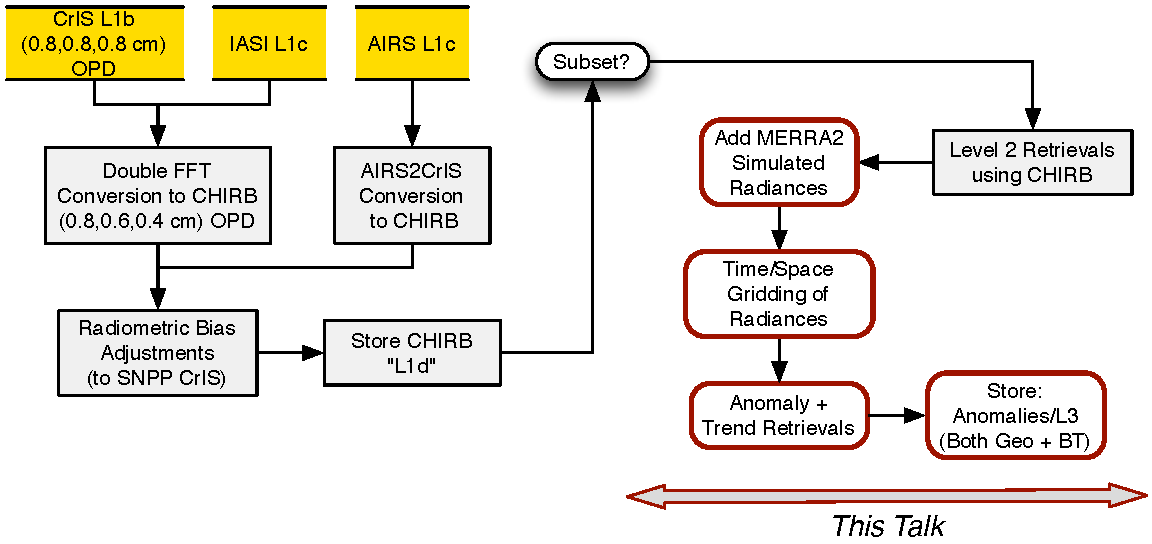
\includegraphics[width=1.0\linewidth]{./airs2cris_stm_talk2_landscape.pdf}
\end{center}



CHIRB: (Common or Climate) Hyperspectral InfraRed Basis

0.8 /0.6 /04  

0.0625 / 0.0833  /  0.1250
\end{frame}

\begin{frame}[label={sec:orga66d60d}]{Introduction}
\vspace{-0.1in}
\begin{center}
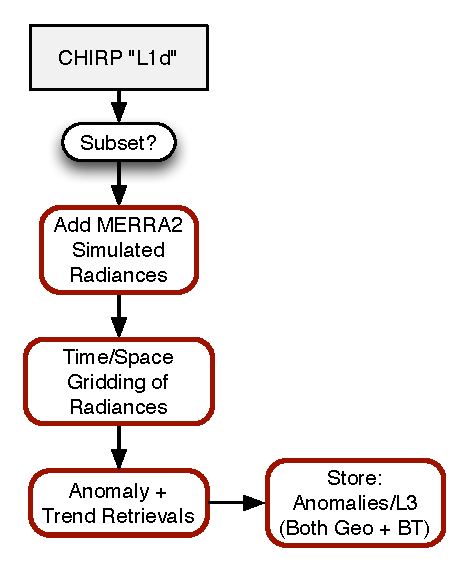
\includegraphics[width=0.6\linewidth]{./airs2cris_stm_talk2_small.pdf}
\end{center}
\end{frame}





\begin{frame}[shrink=10,label={sec:orge01fc6f}]{Overview:  Two Products Proposed}
\vspace{-0.1in}
\begin{block}{(1) Multi-Instrument Hyperspectral Climate Time Series}
\begin{itemize}
\item 1:30 Orbit: AIRS + CrIS, 9:30 Orbit: IASI
\item Convert to common ILS, CrIS 0.8/0.6/0.4 cm OPD (LW/MW/SW) "Hybrid Time Series"
\item Allows inter-instrument radiance calibration, needed for climate
\item Allows use of a common forward model
\item Emphasize routine/fast processing of data for validation and Level 3
\end{itemize}
\end{block}

\begin{block}{(2) Level 3 Products: Radiance and Geophysical}
\begin{itemize}
\item Produce time/space grids of radiance time series and anomalies for climate analysis
\item Generate geophysical (T/Q, etc.) "Level 3" anomaly time series and trends
\item Generating radiance trends/anomalies first reduces errors and influence of a-priori
\item Optimal estimation for Level 2 anomalies, proposal emphasis on applicable covariance estimates and total system uncertainties
\end{itemize}
\end{block}
\end{frame}

\begin{frame}[label={sec:org66ddde2}]{SNPP vs NOAA20 CrIS (via AIRS Snos)}
\vspace{-0.1in}

\begin{center}
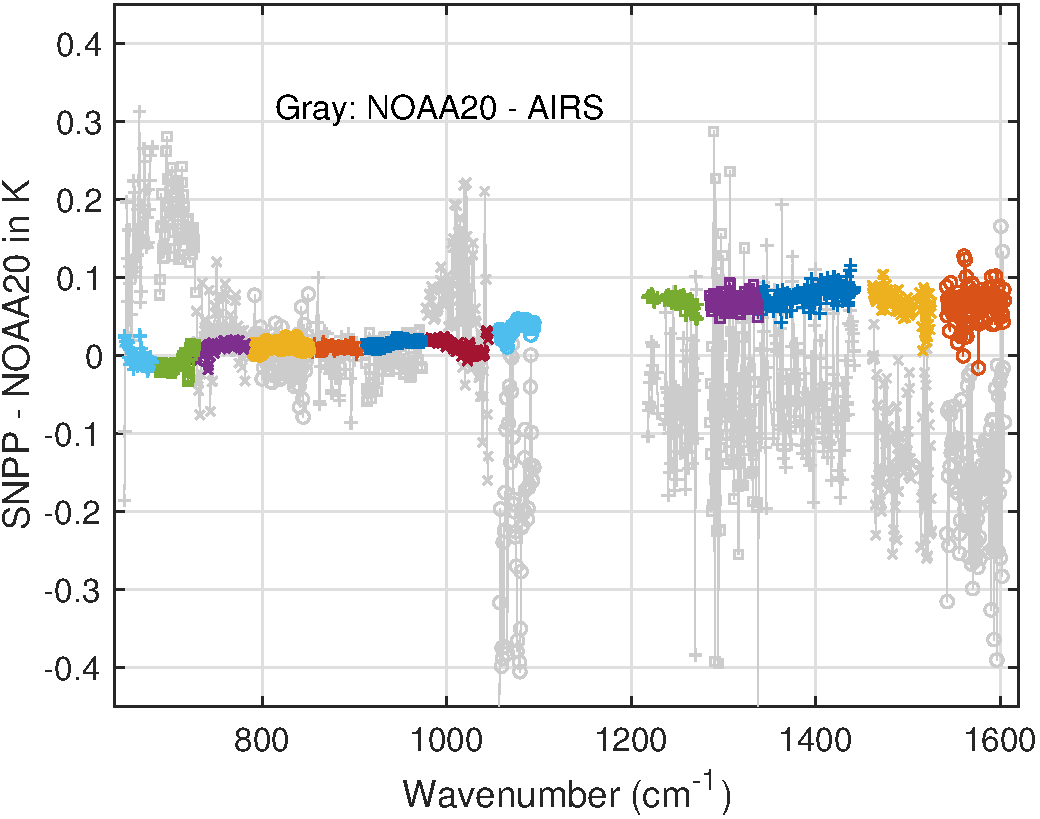
\includegraphics[width=0.7\linewidth]{./oFigs/sno_march2018_snpp_minus_noaa20_with_c2_airs_ingrey.pdf}
\end{center}

\vspace{-0.1in}

\small
\begin{itemize}
\item AIRS and CrIS radiometric calibration differences after putting AIRS on the CrIS ILS grid.  (AIRS - NOAA20 CrIS) and (SNPP CrIS - NOAA20 CrIS) shown.
\end{itemize}
\end{frame}

\begin{frame}[label=flow]{Data Processing Flow}
\vspace{-0.1in}
\begin{center}
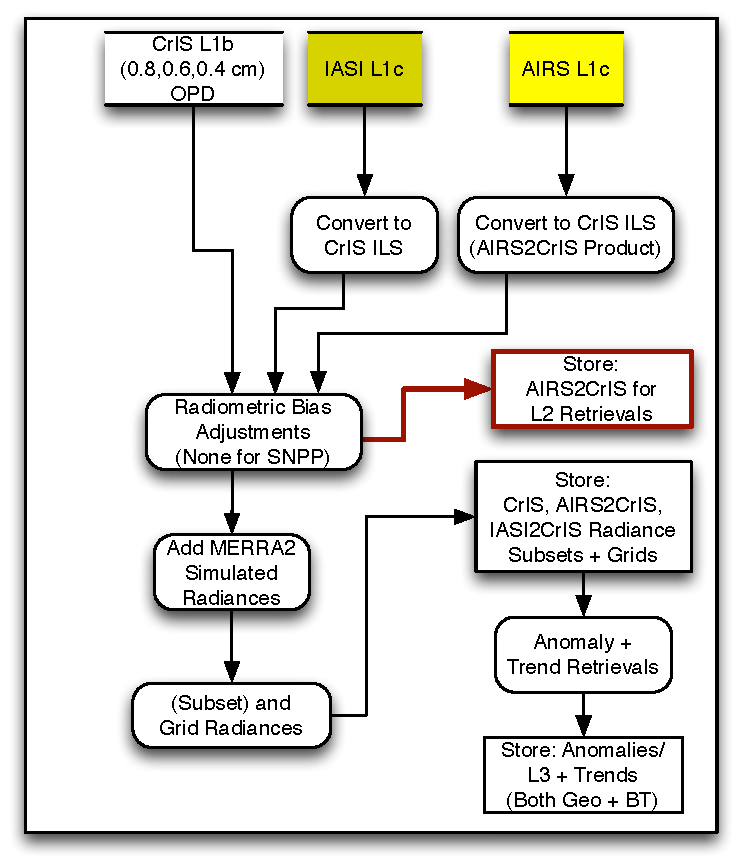
\includegraphics[width=0.64\linewidth]{./oFigs/airs2cris_vx_sounding.pdf}
\end{center}
\end{frame}

\begin{frame}[label={sec:org7fc9b3b}]{AIRS2CrIS for Level 2 Retrievals?  (Summary)}
\begin{itemize}
\item Continuity requires adjusting for satellite differences
\item Only way I can see is to use a common ILS
\item Which allows you to use a common RTA
\item Instrument noises can be adjusted to be identical if needed (AIRS noise will be lowered when converted to CrIS ILS)
\item DOFs of CrIS (NSR or FSR) very similar to AIRS
\item "AIRS2CrIS" product samples will hopefully be ready soon for testing
\end{itemize}
\end{frame}

\begin{frame}[label={sec:org4ebbb7e}]{Example Product Slides Below}
\end{frame}
\begin{frame}[label={sec:org5300dbf}]{Global B(T) Trend (hardest case)}
\vspace{-0.15in}
\begin{center}
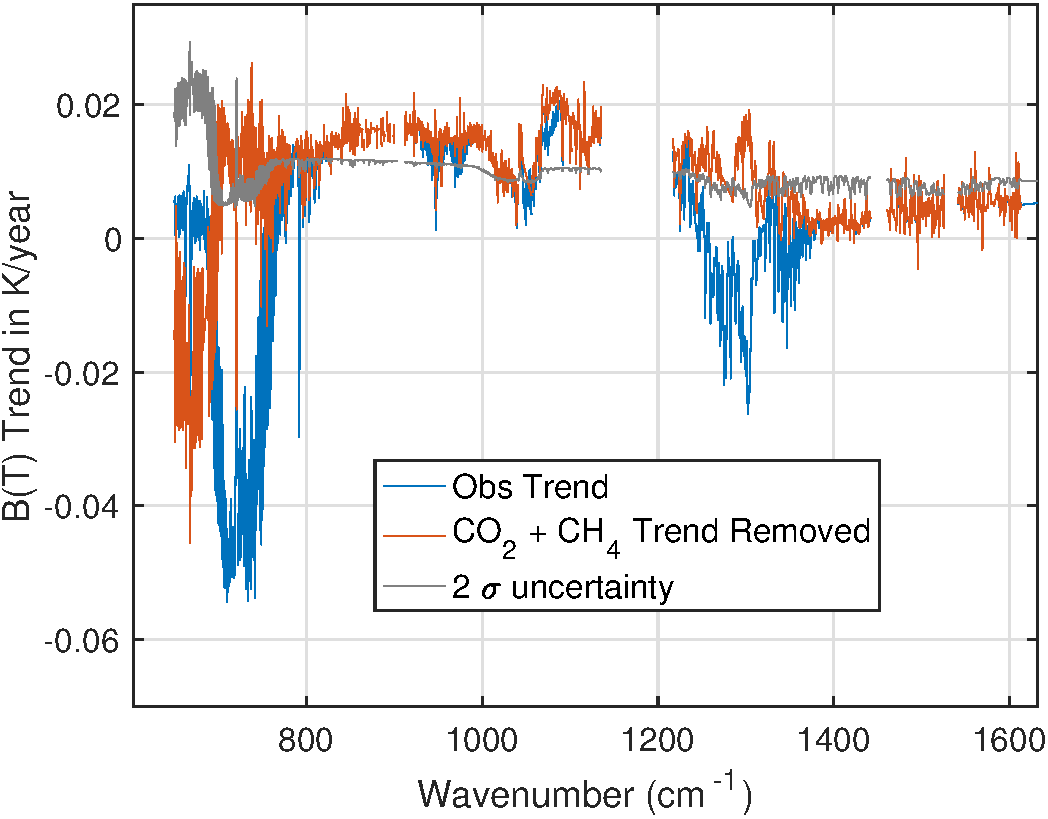
\includegraphics[width=0.8\linewidth]{./oFigs/airs_14year_global_trends.pdf}
\end{center}

\small
Uncertain on fit vs specify \cd, \methane etc. trends. We have done both.

Specifying OK for long-term trends.  
\end{frame}

\begin{frame}[label={sec:orgfb121a1}]{Example: 14-Year Zonal Temperature Trends}
\vspace{-0.1in}

\small \emph{NOTE larger color scale on left.}

\vspace{-0.1in}

\begin{columns}
\begin{column}{0.55\columnwidth}
\begin{block}{\footnotesize From Level 3}
\begin{center}
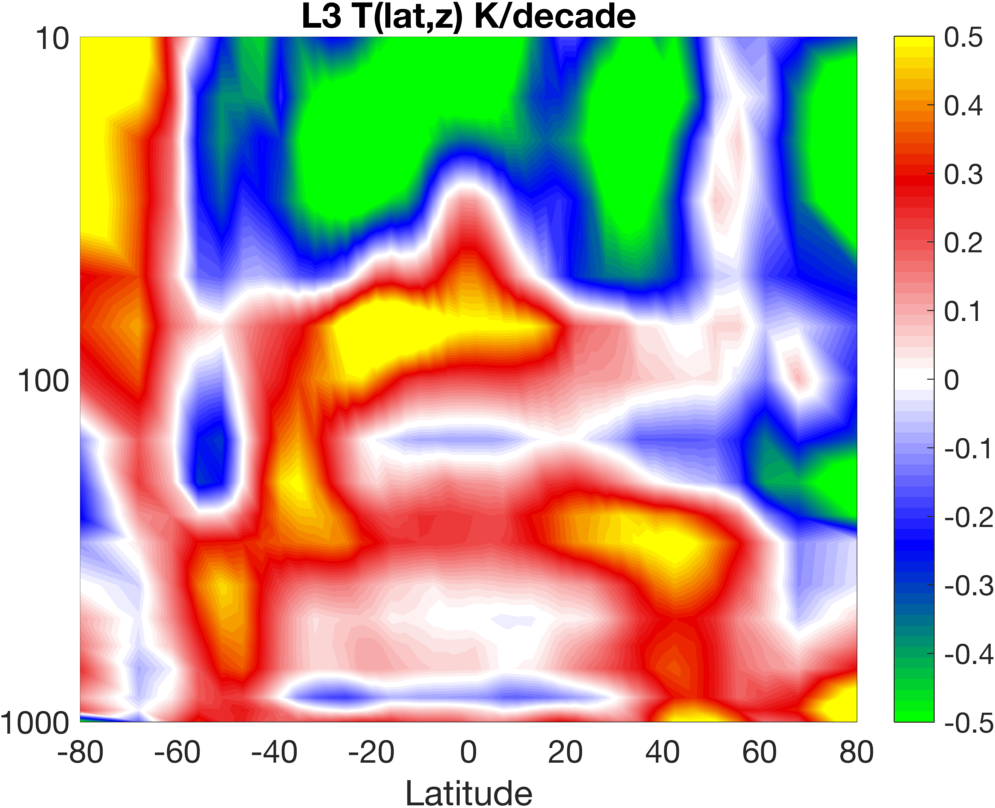
\includegraphics[width=\linewidth]{./oFigs/final_l3_t.png}
\end{center}
\end{block}
\end{column}

\begin{column}{0.55\columnwidth}
\begin{block}{\footnotesize From Radiance Derivatives}
\begin{center}
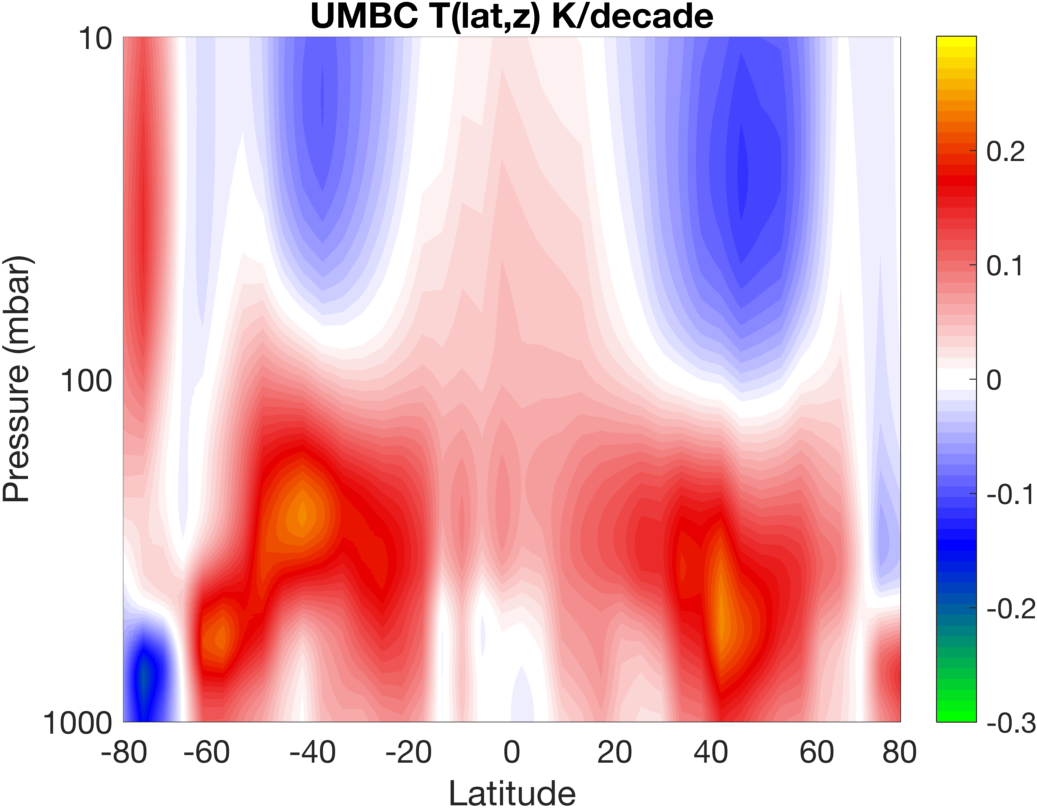
\includegraphics[width=\linewidth]{./oFigs/final_umbc_t_zoom_cmap.png}
\end{center}
\end{block}
\end{column}
\end{columns}

Interannual variability (observation covariance) regularizes OE solution.

Need to work on off-diagonal obs covariances to get uncertainties right.
\end{frame}

\begin{frame}[label={sec:orgaec1bb4}]{Anomaly Example: Water Vapor (27N to 30N Latitude Zonal)}
\vspace{-0.35in}

\begin{columns}
\begin{column}{0.55\columnwidth}
\begin{block}{\footnotesize From radiance anomaly}
\vspace{-0.1in}
\begin{center}
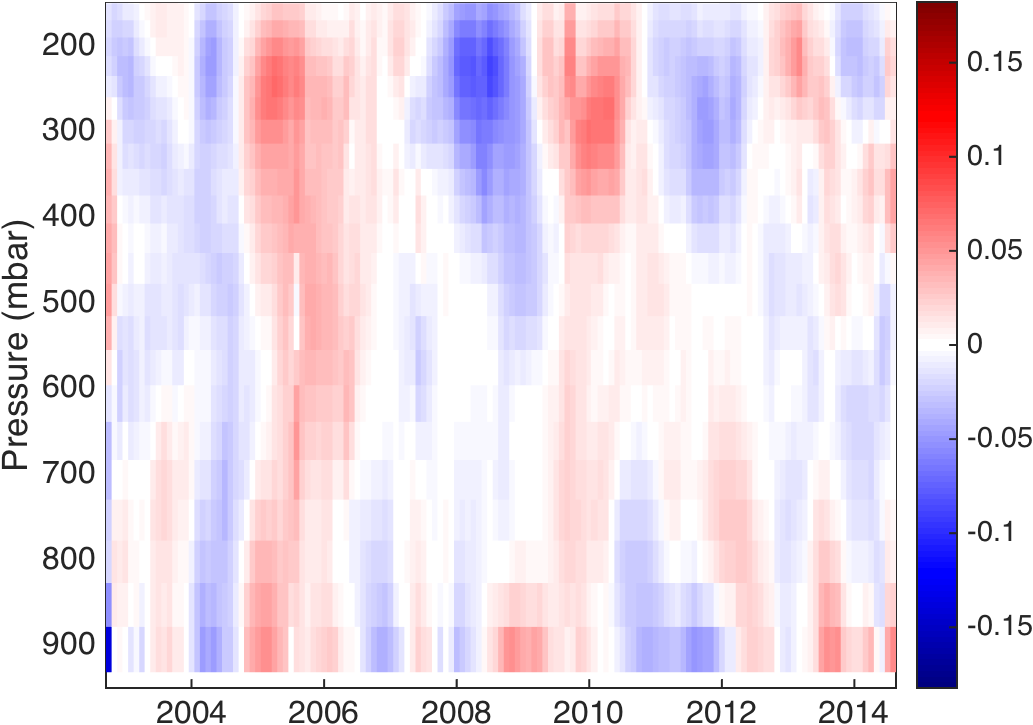
\includegraphics[width=0.8\linewidth]{./oFigs/water_lati_30_UMBC.png}
\end{center}
\end{block}
\end{column}

\begin{column}{0.55\columnwidth}
\begin{block}{\footnotesize ERA \(\times\) Avg Kernel}
\vspace{-0.1in}
\begin{center}
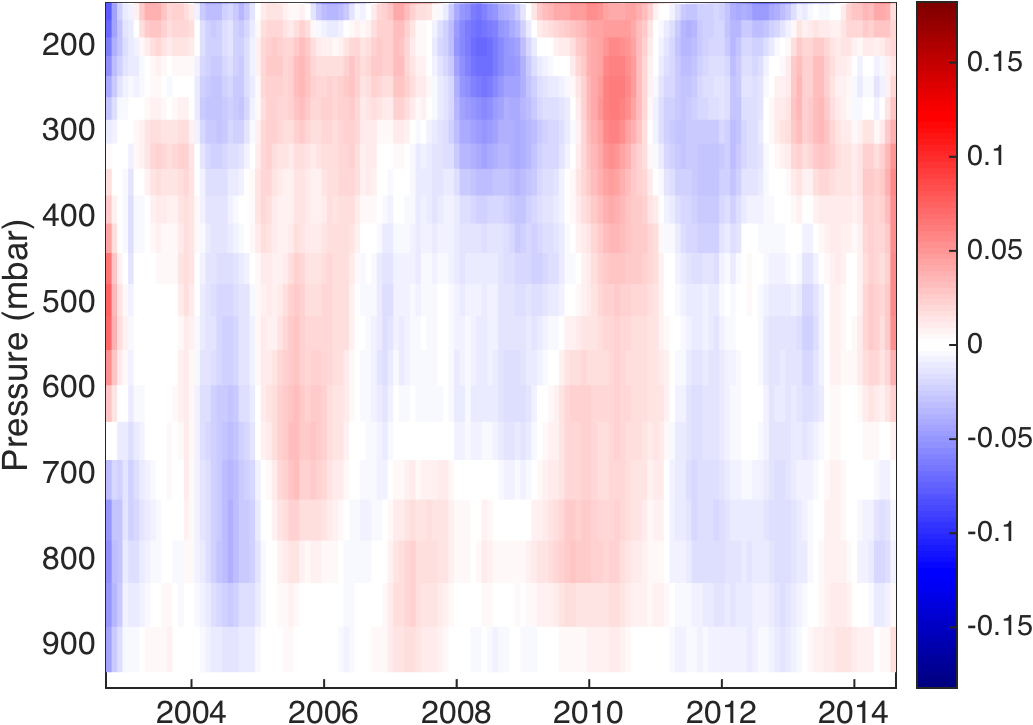
\includegraphics[width=0.8\linewidth]{./oFigs/water_lati_30_ERA.png}
\end{center}
\end{block}
\end{column}
\end{columns}

\vspace{-0.15in}
\begin{columns}
\begin{column}{0.55\columnwidth}
\begin{block}{\footnotesize AIRS Level 3}
\vspace{-0.1in}
\begin{center}
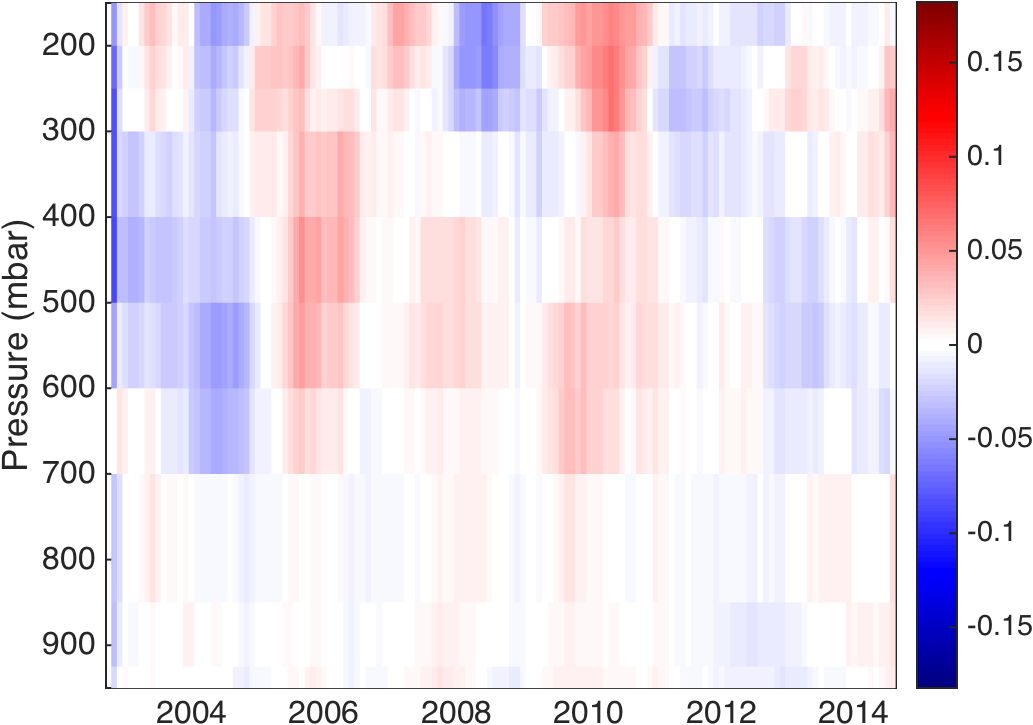
\includegraphics[width=0.8\linewidth]{./oFigs/water_lati_30_L3.png}
\end{center}
\end{block}
\end{column}
\end{columns}
\end{frame}
\end{document}